\section{Architettura del sistema e tecnologie usate}
Nel contesto del progetto PANTHEON la presente relazione descrive una possibile implementazione di un sistema di monitoraggio nel contesto del \textit{Data Collection and Pre-processing layer} (si veda il paragrafo \ref{pantheon-architecture}).\par

Il codice del progetto realizzato è open-source ed è disponibile presso il seguente link: \url{https://github.com/bug-data/Big_Data_Second_Project}.\par

Nello specifico è stato realizzato un sistema che acquisisce dati dai ``sensori'' (in realtà dai file csv a disposizione), li processa, li salva su un database e infine visualizza i dati memorizzati su browser in tempo reale.\par

Al fine di realizzare questo sistema è stato utilizzato \textit{docker compose} \\
(\url{https://docs.docker.com/compose}), uno strumento per la \textit{composizione} di contenitori, ovvero uno strumento che consente di realizzare applicazioni composte da più contenitori che comunicano tra loro.\par

In particolare, grazie a docker compose, i vari servizi che compongono il sistema realizzato (come il servizio di processamento dei dati e il servizio di memorizzazione dei dati) sono stati eseguiti come dei \textit{container Docker} e collegati tramite una rete virtuale che consente ai container di poter interagire tra loro.\par

Di seguito si riporta schematicamente l'architettura del sistema realizzato.

\begin{figure}[ht]
\centering
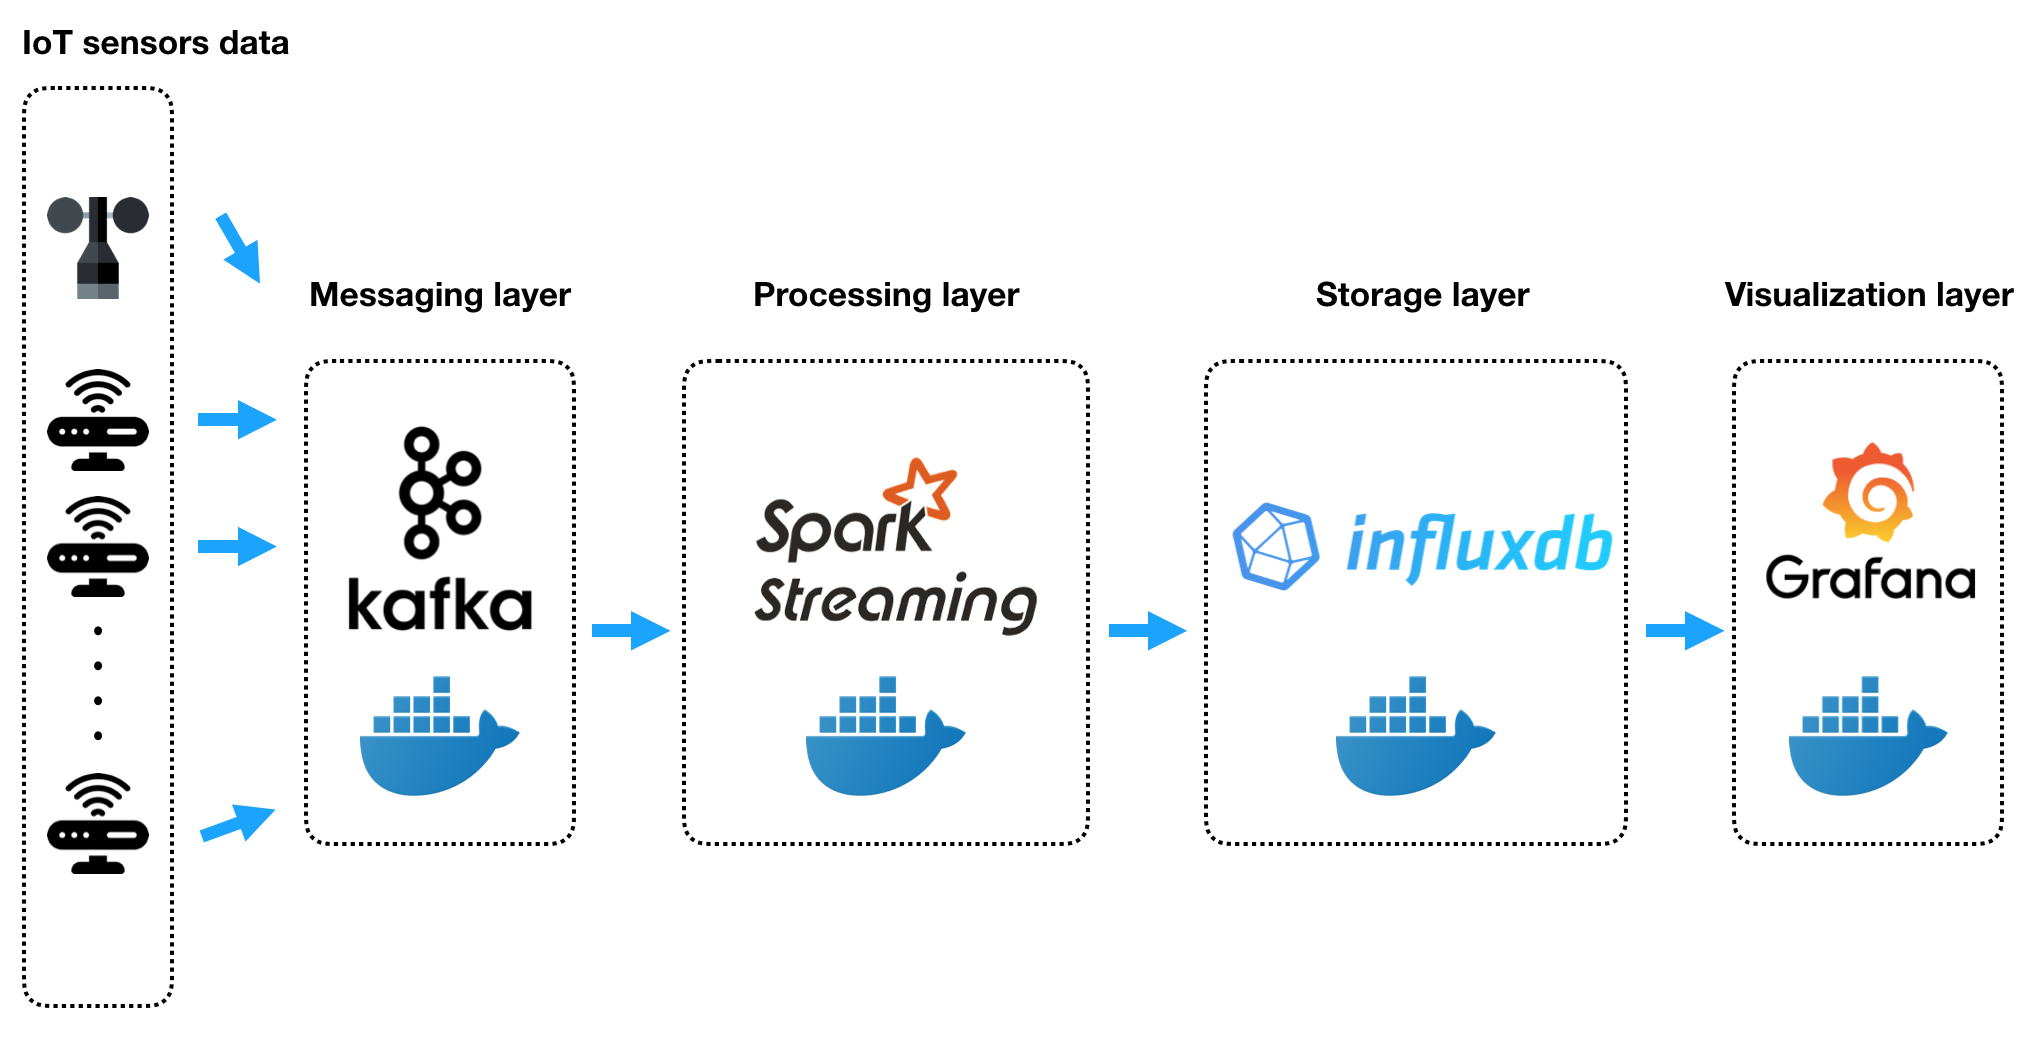
\includegraphics[width=1\textwidth]{project-architecture}
\caption{Rappresentazione schematica del sistema di monitoraggio realizzato}
\label{fig:project-architecture}
\end{figure}

Dunque il sistema realizzato è composto fondamentalmente da 5 blocchi:

\begin{itemize}
    \item \textit{IoT sensors data}, che sono i sensori installati nel noccioleto, i quali rilevano dati che vengono poi inviati al blocco successivo. Come si è detto in precedenza abbiamo simulato la presenza di questi sensori trasmettendo le righe dei file a disposizione al blocco successivo dell'architettura;
    \item \textit{Messaging layer}, che si occupa di memorizzare i dati/messaggi provenienti dai sensori (leggasi file csv) per poi fornirli al blocco che si occupa del processamento dei dati;
    \item \textit{Processing layer}, che si occupa di processare in tempo reale i dati provenienti dal messaging layer;
    \item \textit{Storage layer}, che si occupa di memorizzare i dati processati dal blocco precedente;
    \item \textit{Visualization layer}, che si occupa di visualizzare i dati memorizzati in tempo reale.
\end{itemize}{}

Nelle sezioni a seguire verranno descritti più in dettaglio i blocchi che compongono l'architettura in figura \ref{fig:project-architecture}.

\subsection{Dati prodotti dai sensori IoT}
Come detto in precedenza nel paragrafo \ref{dati-a-disposizione}, sono stati messi a disposizione, ai fini del progetto, dati provenienti sia dalla stazione meteo che dai sensori installati a terra, che misurano l'umidità e la temperatura del terreno.\par

Al fine di simulare l'invio di dati dai sensori al messagging layer (realizzato usando Kafka), è stato realizzato uno script, scritto in Python, che legge ciascuna riga del file in input, la converte in un JSON (usando come chiavi del JSON gli stessi campi riportati nel file csv in input) e lo trasmette al container su cui è in esecuzione Kafka (raggiungibile all'endpoint \texttt{kafka:9092}) ad intervalli di 1 secondo. Lo script in questione è stato poi eseguito fornendo in input i file \texttt{pantheon20190612-stazione.csv} e \texttt{pantheon20190612-nodi.csv}.\par

Per consentire allo script Python di poter interagire con Kafka è stato utilizzato il package \textit{kafka-python} (\url{https://github.com/dpkp/kafka-python}) che consiste in un client Kafka per il linguaggio Python.

\subsection{Messaging layer}
I messaggi trasmessi attraverso lo script Python descritto in precedenza giungono quindi al messaging layer, realizzato con Kafka. Il vantaggio di usare un blocco intermedio tra i produttori di dati (sensori IoT) e i consumatori (Spark Streaming) sta nella possibilità di disaccopiare gli uni dagli altri. Ad esempio, grazie a questo strato intermedio, sarebbe possibile utilizzare una diversa tecnologia per processare gli stream di dati prodotti dai sensori (ad esempio Apache Storm) senza che questo abbia alcun impatto sui produttori di dati. In assenza di questa indirezione offerta da Kafka sarebbe stato necessario configurare i sensori affinché inviassero dati al cluster su cui è in esecuzione Apache Storm.\par

Tornando alla descrizione dell'architettura del sistema realizzato, come detto in precedenza, i messaggi prodotti dallo script Python vengono poi trasmessi e memorizzati in un container su cui è in esecuzione Kafka.\par

In particolare i messaggi provenienti dalla stazione meteo e dai nodi vengono memorizzati in \textit{topic} differenti. Più precisamente, all'avvio del contenitore su cui è in esecuzione Kafka, vengono configurati 10 topic, di cui 1 per la stazione (\texttt{weather}) e 9 per ciascun nodo o sensore (\texttt{nodeN}, dove N è l'identificativo del nodo, e.g. \texttt{node1}, \texttt{node2} ecc.).\par

I topic sono stati configurati a mezzo della variabile d'ambiente \\ \texttt{KAFKA\_CREATE\_TOPICS} e ciascun topic ha un fattore di replicazione pari ad 1 (solo per fini di test) ed un numero di partizioni pari ad 1 (per preservare l'ordine temporale in cui vengono ricevuti i dati quando quest'ultimi vengono passati al processing layer).

\subsection{Processing layer}
I dati memorizzati su Kafka vengono poi inviati ad un cluster di container Spark composti da un singolo \textit{master} e da un singolo \textit{worker}. Il processamento dei dati avviene tramite Spark Streaming. Gli script per processare i dati sono stati realizzati in Python.\par

Al fine di poter leggere lo stream di dati memorizzato in Kafka si è fatto ricorso alla libreria Java \textit{spark-streaming-kafka}.\par

Per quanto riguarda il processamento dei dati, durante l'esecuzione dello script Spark vengono letti da Kafka i messaggi provenienti dai 10 topic configurati in precedenza. Tali dati confluiscono poi in input a Spark Streaming come uno stream di dati. La durata dei \textit{minibatch} di dati su cui opera Spark Streaming è stata configurata a 10 secondi.\par

Successivamente i dati vengono aggregati in base al topic, per poi procedere effettivamente con l'elaborazione vera  e propria dei dati. In particolare per ciacun minibatch viene calcolato il valore medio di ciascun campo di ciascun topic (al fine di ridurre la mole di dati da salvare sullo storage layer) e vengono calcolati ulteriori parametri come ad esempio l'escursione termica.\par

Infine, i dati così processati vengono salvati sullo storage layer, che consiste in un container su cui è installato InfluxDB. Il salvataggio dei dati prodotti da Spark Streaming su InfluxDB avviene a mezzo del package Python \textit{influxdb} (\url{https://pypi.org/project/influxdb/}).

\subsection{Storage layer}
InfluxDB è un base di dati che appartiene alla categoria dei \textit{Time Series Database (TSDB)}, ovvero una tipologia di  database ottimizzati per \textit{time series data}. I time series data sono dati o eventi che vengono registrati, aggregati e monitorati nel tempo, come ad esempio la quantità di CPU e RAM usata in un server, i dati provenienti da sensori, o ancora le transazioni effettuate in borsa e così via.\par

Tipicamente queste tipologie di dati sono accomunate da analoghe elaborazioni. Difatti i dati relativi ad eventi che sono avvenuti in tempi non molto recenti vengono spesso aggregati al fine di ridurre lo spazio su disco o addirittura cancellati perché non più necessari. Allo stesso modo, queste tipologie di dati vengono letti specificando spesso un intervallo di tempo.

Un time series database è una particolare tipologia di basi di dati per la memorizzazione di misure o eventi che sono associati ad un timestamp ed è ottimizzato per misurare i cambiamenti nel tempo di una data metrica (come ad esempio la percentuale di CPU utilizzata nell'esempio precedente).

Notare come nell'ultimo anno i TSDB siano stati la categoria di database a maggiore crescita in termini di popolarità secondo DB-Engines \\ (\url{https://db-engines.com/en/ranking_categories})

\begin{figure}[ht]
\centering
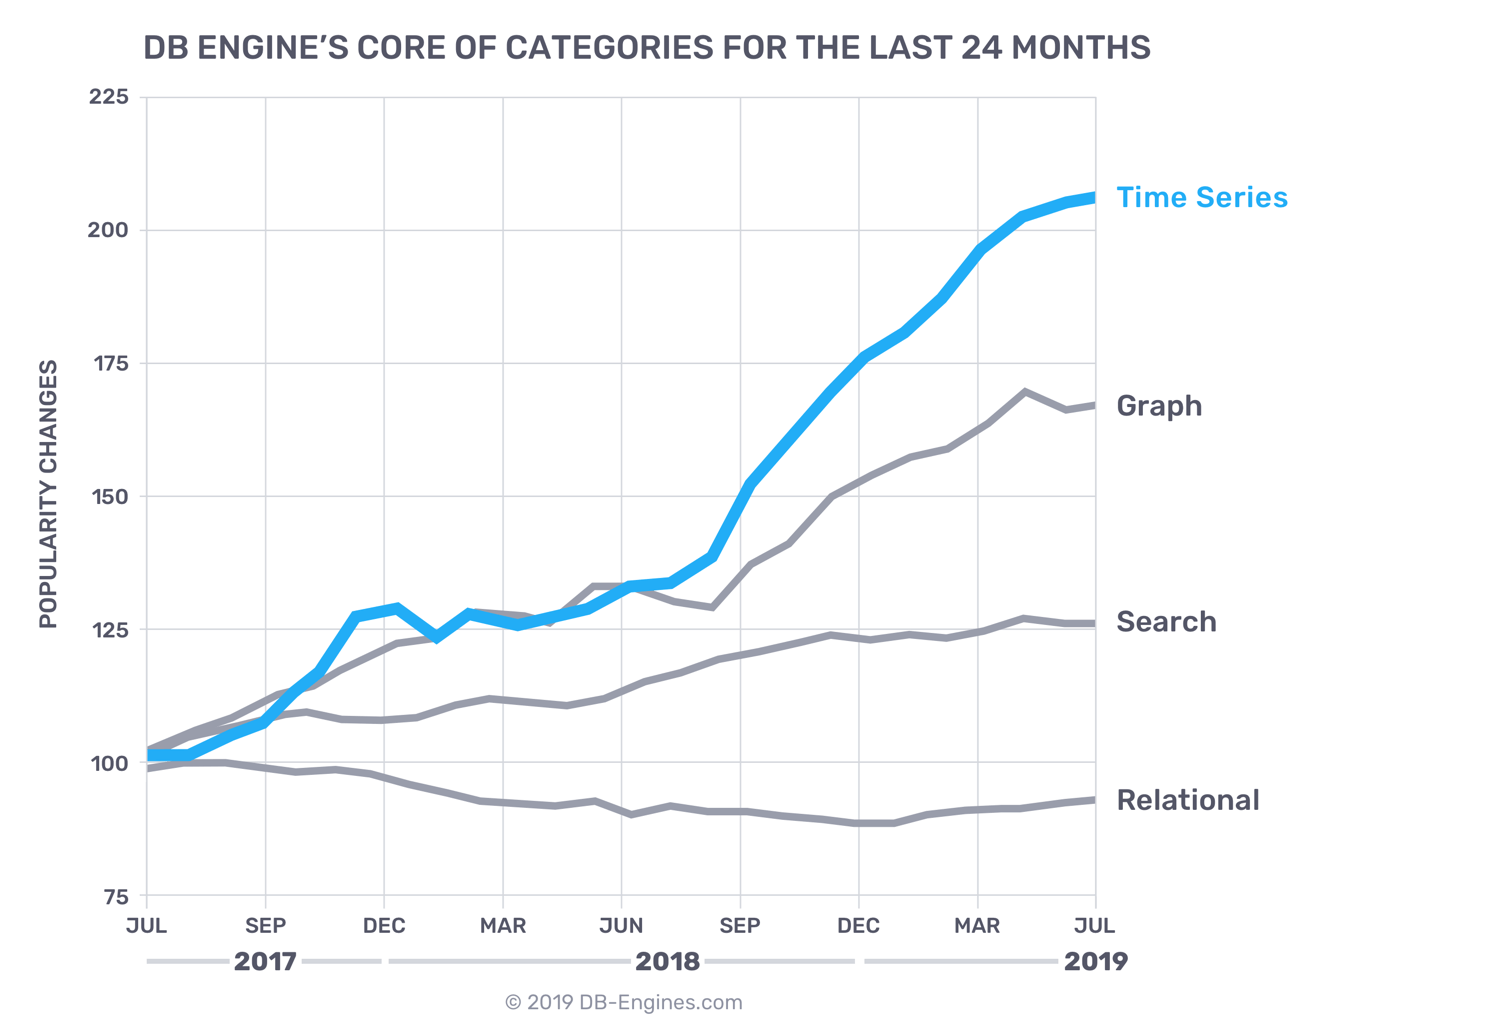
\includegraphics[width=0.9\textwidth]{db-model-trend}
\caption{Trend dei diversi modelli di database nell'ultimo anno in termini di popolarità}
\label{fig:db-model-trend}
\end{figure}

Dunque i TSBD sembrano prestarsi bene al contesto in cui si è svolto il progetto descritto nella presente relazione e questo ci ha portato a selezionare un TSDB per memorizzare i dati prodotti da Spark Streaming.\par

Nel panorama dei TSDB la nostra scelta è poi ricaduta su InfluxDB. Questa scelta è motivata dalle seguenti ragioni:

\begin{itemize}
    \item Popolarità: tra i time-series databases, InfluxDB si classifica al primo posto secondo DB-Engines (figura \ref{fig:tsdbms-rank}), cosa che può suggerire il fatto che si tratta di una tecnologia matura
    \item Compatibilità con \textit{Grafana} (che verrà descritto nella sezione successiva)
\end{itemize}

\begin{figure}[ht]
\centering
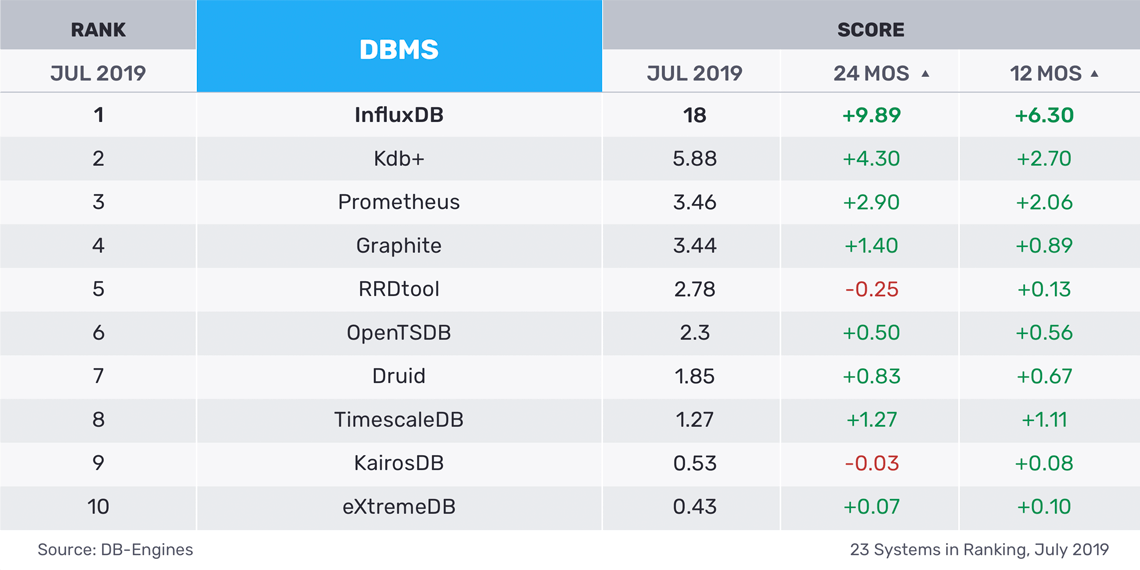
\includegraphics[width=1\textwidth]{tdbms-rank}
\caption{Ranking dei TSDMB secondo DB-Engines}
\label{fig:tsdbms-rank}
\end{figure}

Si riportano di seguito i concetti di base di InfluxDB:\par

\begin{itemize}
    \item \textit{Measurement}, che corrisponde al concetto di \textit{tabella} in un RDBMS;
    \item \textit{Tag}, che può essere visto come una colonna indicizzata in un RDBMS (ad esempio un tag potrebbe corrispondere all'identificativo di ciascuno dei 9 nodi/sensori);
    \item \textit{Field}, che corrisponde al concetto di colonna (non indicizzata) in un RDBMS;
    \item \textit{Point}, che corrisponde al concetto di riga in un RDBMS.
\end{itemize}{}

Si riporta di seguito una sequenza di dati di esempio rappresentati sia in un RDBMS che in InfluxDB:\par

\begin{figure}[ht]
\centering
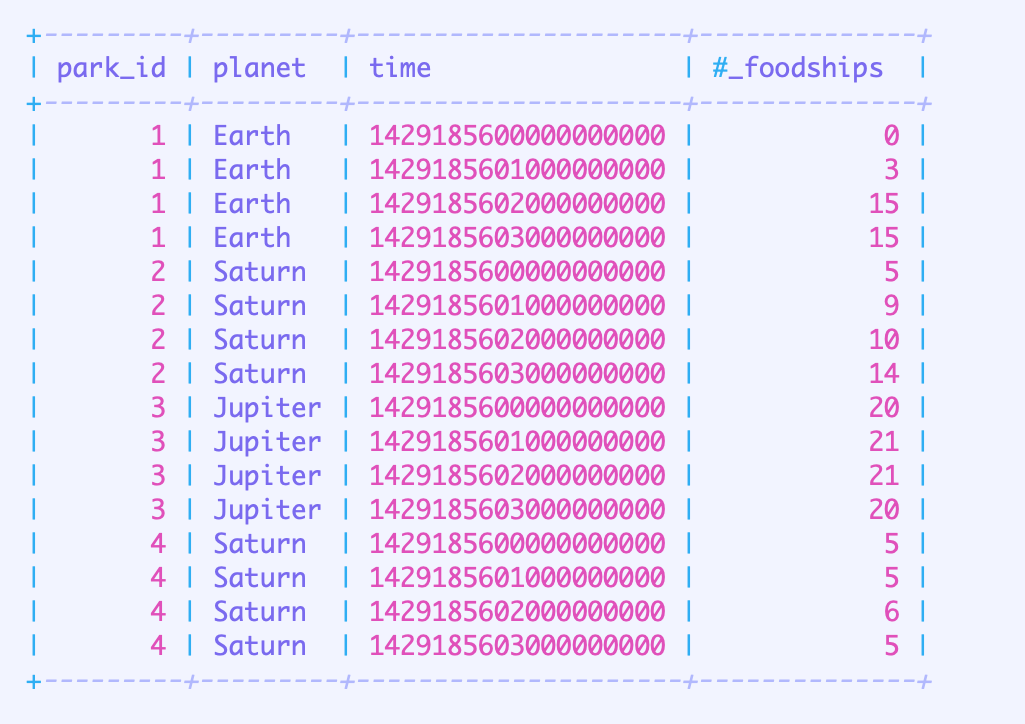
\includegraphics[width=1\textwidth]{rdbms-table}
\caption{Esempio di dati memorizzati in un RDBMS}
\label{fig:rdbms-table}
\end{figure}

\begin{figure}[ht]
\centering
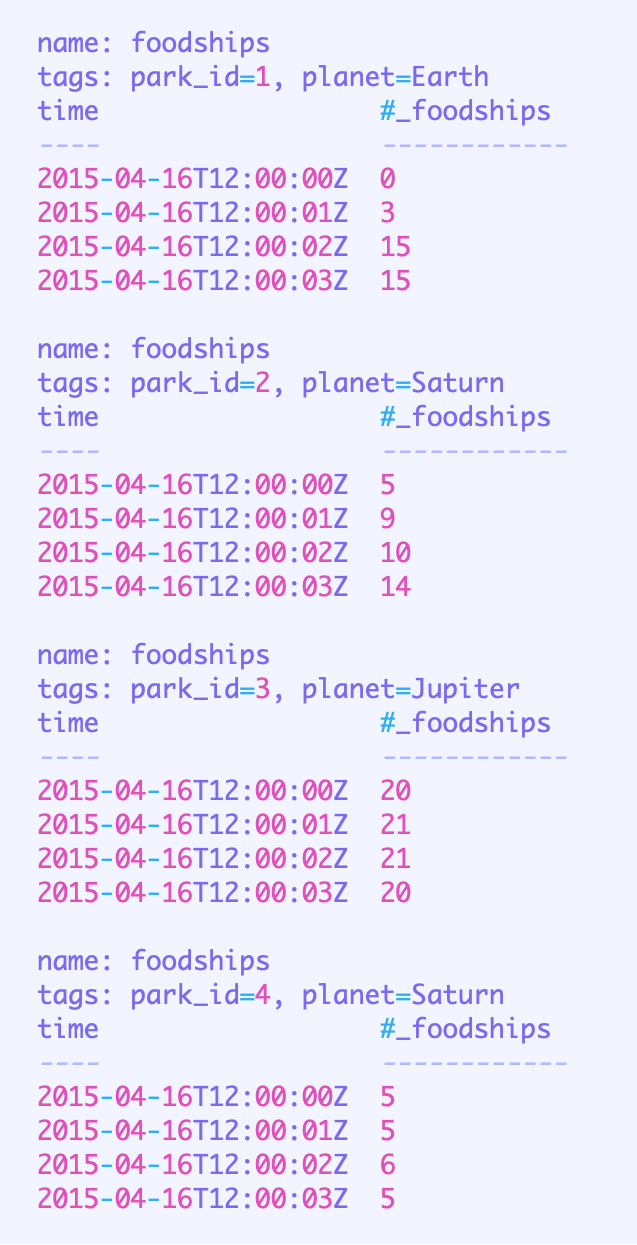
\includegraphics[width=0.7\textwidth]{influxdb-table}
\caption{Esempio di dati memorizzati in InfluxDB}
\label{fig:influxdb-table}
\end{figure}

\clearpage

Con riferimento ad InfluxDB in questo esempio:

\begin{itemize}
    \item \texttt{foodship} corrisponde alla measurement
    \item \texttt{park\_id} e \texttt{planet} sono i tag
    \item \texttt{\#\_foodships} corrisponde ad un field
\end{itemize}



Notare come in InfluxDB sia presente per ciascuna riga una colonna aggiuntiva, di nome \texttt{time} che rappresenta un timestap associato alla riga in questione.\par

Per quanto riguarda i dati processati da Spark Streaming, questi sono stati salvati in due measurement distinte: \par

\begin{itemize}
    \item \texttt{Stazioni}, che contiene i dati processati da Spark Streaming relativi alla stazione meteo. In particolare sono stati creati tanti field quanti sono i campi processati da Spark relativamente alla stazione meteo (ad esempio \texttt{temp1\_min}, \texttt{temp1\_max} ecc.). Inoltre è stato utilizzato l'identificatore di riga (campo \texttt{id\_dato} dei file csv) come tag.
    \item \texttt{Nodi}, che contiene i dati processati da Spark Streaming relativi ai sensori/nodi. In particolare i dati dei vari sensori vengono distinti a mezzo di tag della forma \texttt{nodeN} (e.g. \texttt{node1} per il primo nodo, \texttt{node2} per il secondo e così via). I field della measurement corrispondono ai campi che sono stati processati con Spark Streaming (ad esempio \texttt{soil\_0\_water\_content}, \texttt{soil\_1\_water\_content} ecc.)
\end{itemize}{}

\clearpage

\begin{figure}[ht]
\centering
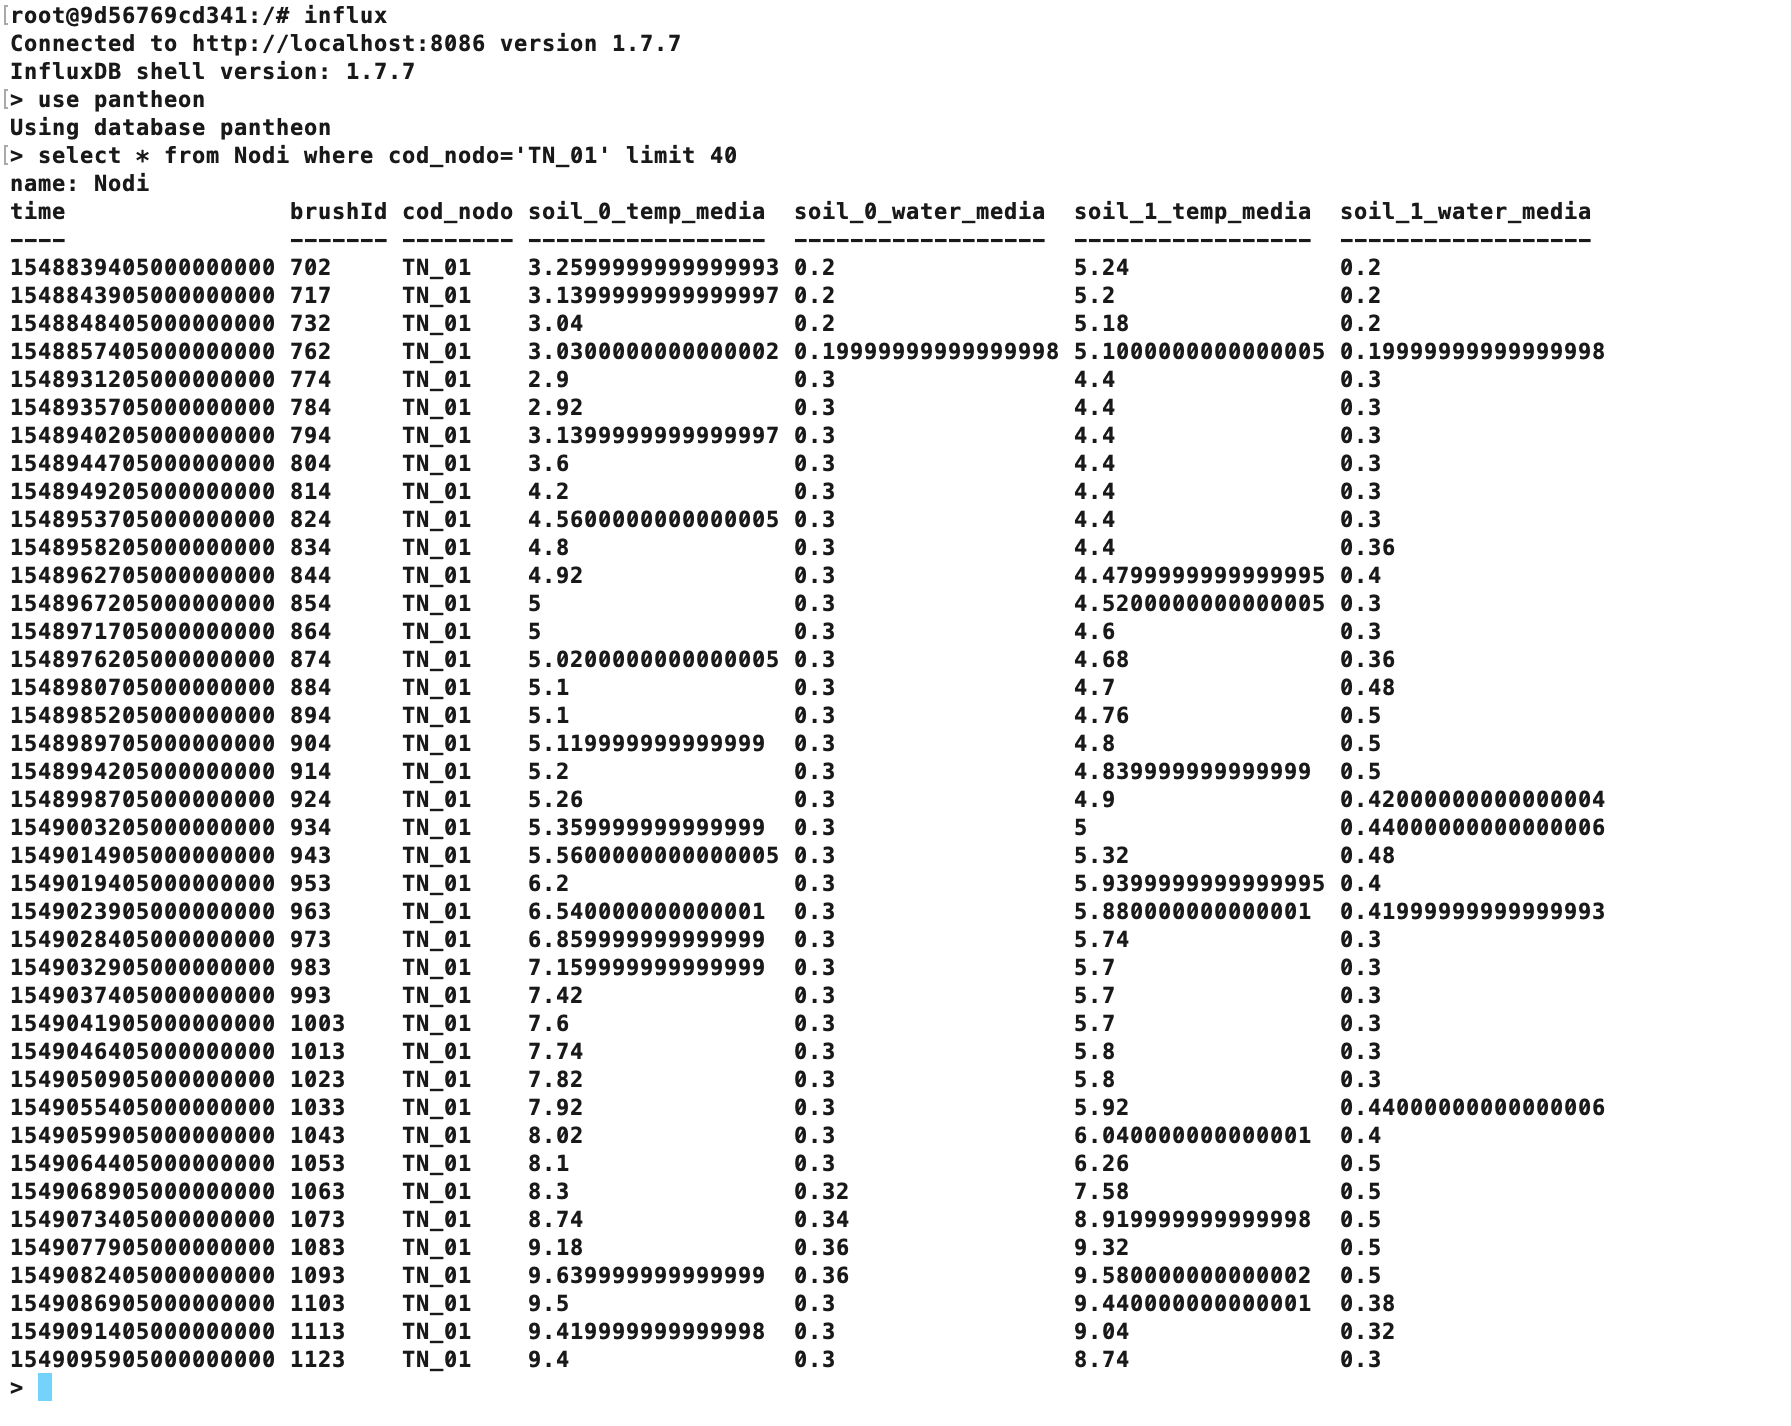
\includegraphics[width=1\textwidth]{influxdb-node1-table}
\caption{Prime 40 righe della tabella Nodi contenente i dati processati per il nodo con identificativo ``TN\_01''}
\label{fig:influxdb-node1-table}
\end{figure}

\clearpage

\subsection{Visualization layer}
Infine per visualizzare i dati che vengono periodicamente memorizzati in InfluxDB è stato impiegato Grafana. Si tratta di uno strumenti di visualizzazione di serie temporali, accessibile tramite browser, che supporta una serie di database da cui leggere i dati quali \textit{Graphite}, \textit{MySQL}, \textit{PostgreSQL}, \textit{ElasticSearch} e molti altri oltre al già citato InfluxDB.\par

In particolare grazie a Grafana è stata realizzata una \textit{dashboard} in cui sono state riportate le serie temporali associati a ciascuno dei campi processati tramite Spark Streaming e memorizzati in InfluxDB. Si riporta di seguito una porzione della dashboard realizzata. \par

Si precisa come di default Grafana richieda all'avvio di effettuare il login (lo username e la password di default sono \textit{admin}, \textit{admin}) di specificare la sorgente da cui leggere i dati (nel nostro caso InfluxDB) per poi realizzare la dashboard attraverso l'interfaccia grafica di Grafana. Per automatizzare il processo di creazione della dashboard, si è proceduto nella seguente maniera: è stato dapprima creata la dashboard ``a mano'' attraverso l'interfaccia grafica di Grafana, per poi salvarlo in formato JSON (cliccando sulla opzione messa a disposizione da Grafana per esportare le dashboard). Successivamente, modificando opportuni file di configurazione è stato possibile disabilitare ad ogni avvio il login (ai soli fini del progetto) e caricare in automatico la dashboard a partire dal file JSON scaricato in precedenza.\par

Si riporta di seguito una istantanea di una porzione della dashboard realizzata:

\begin{figure}[ht]
\centering
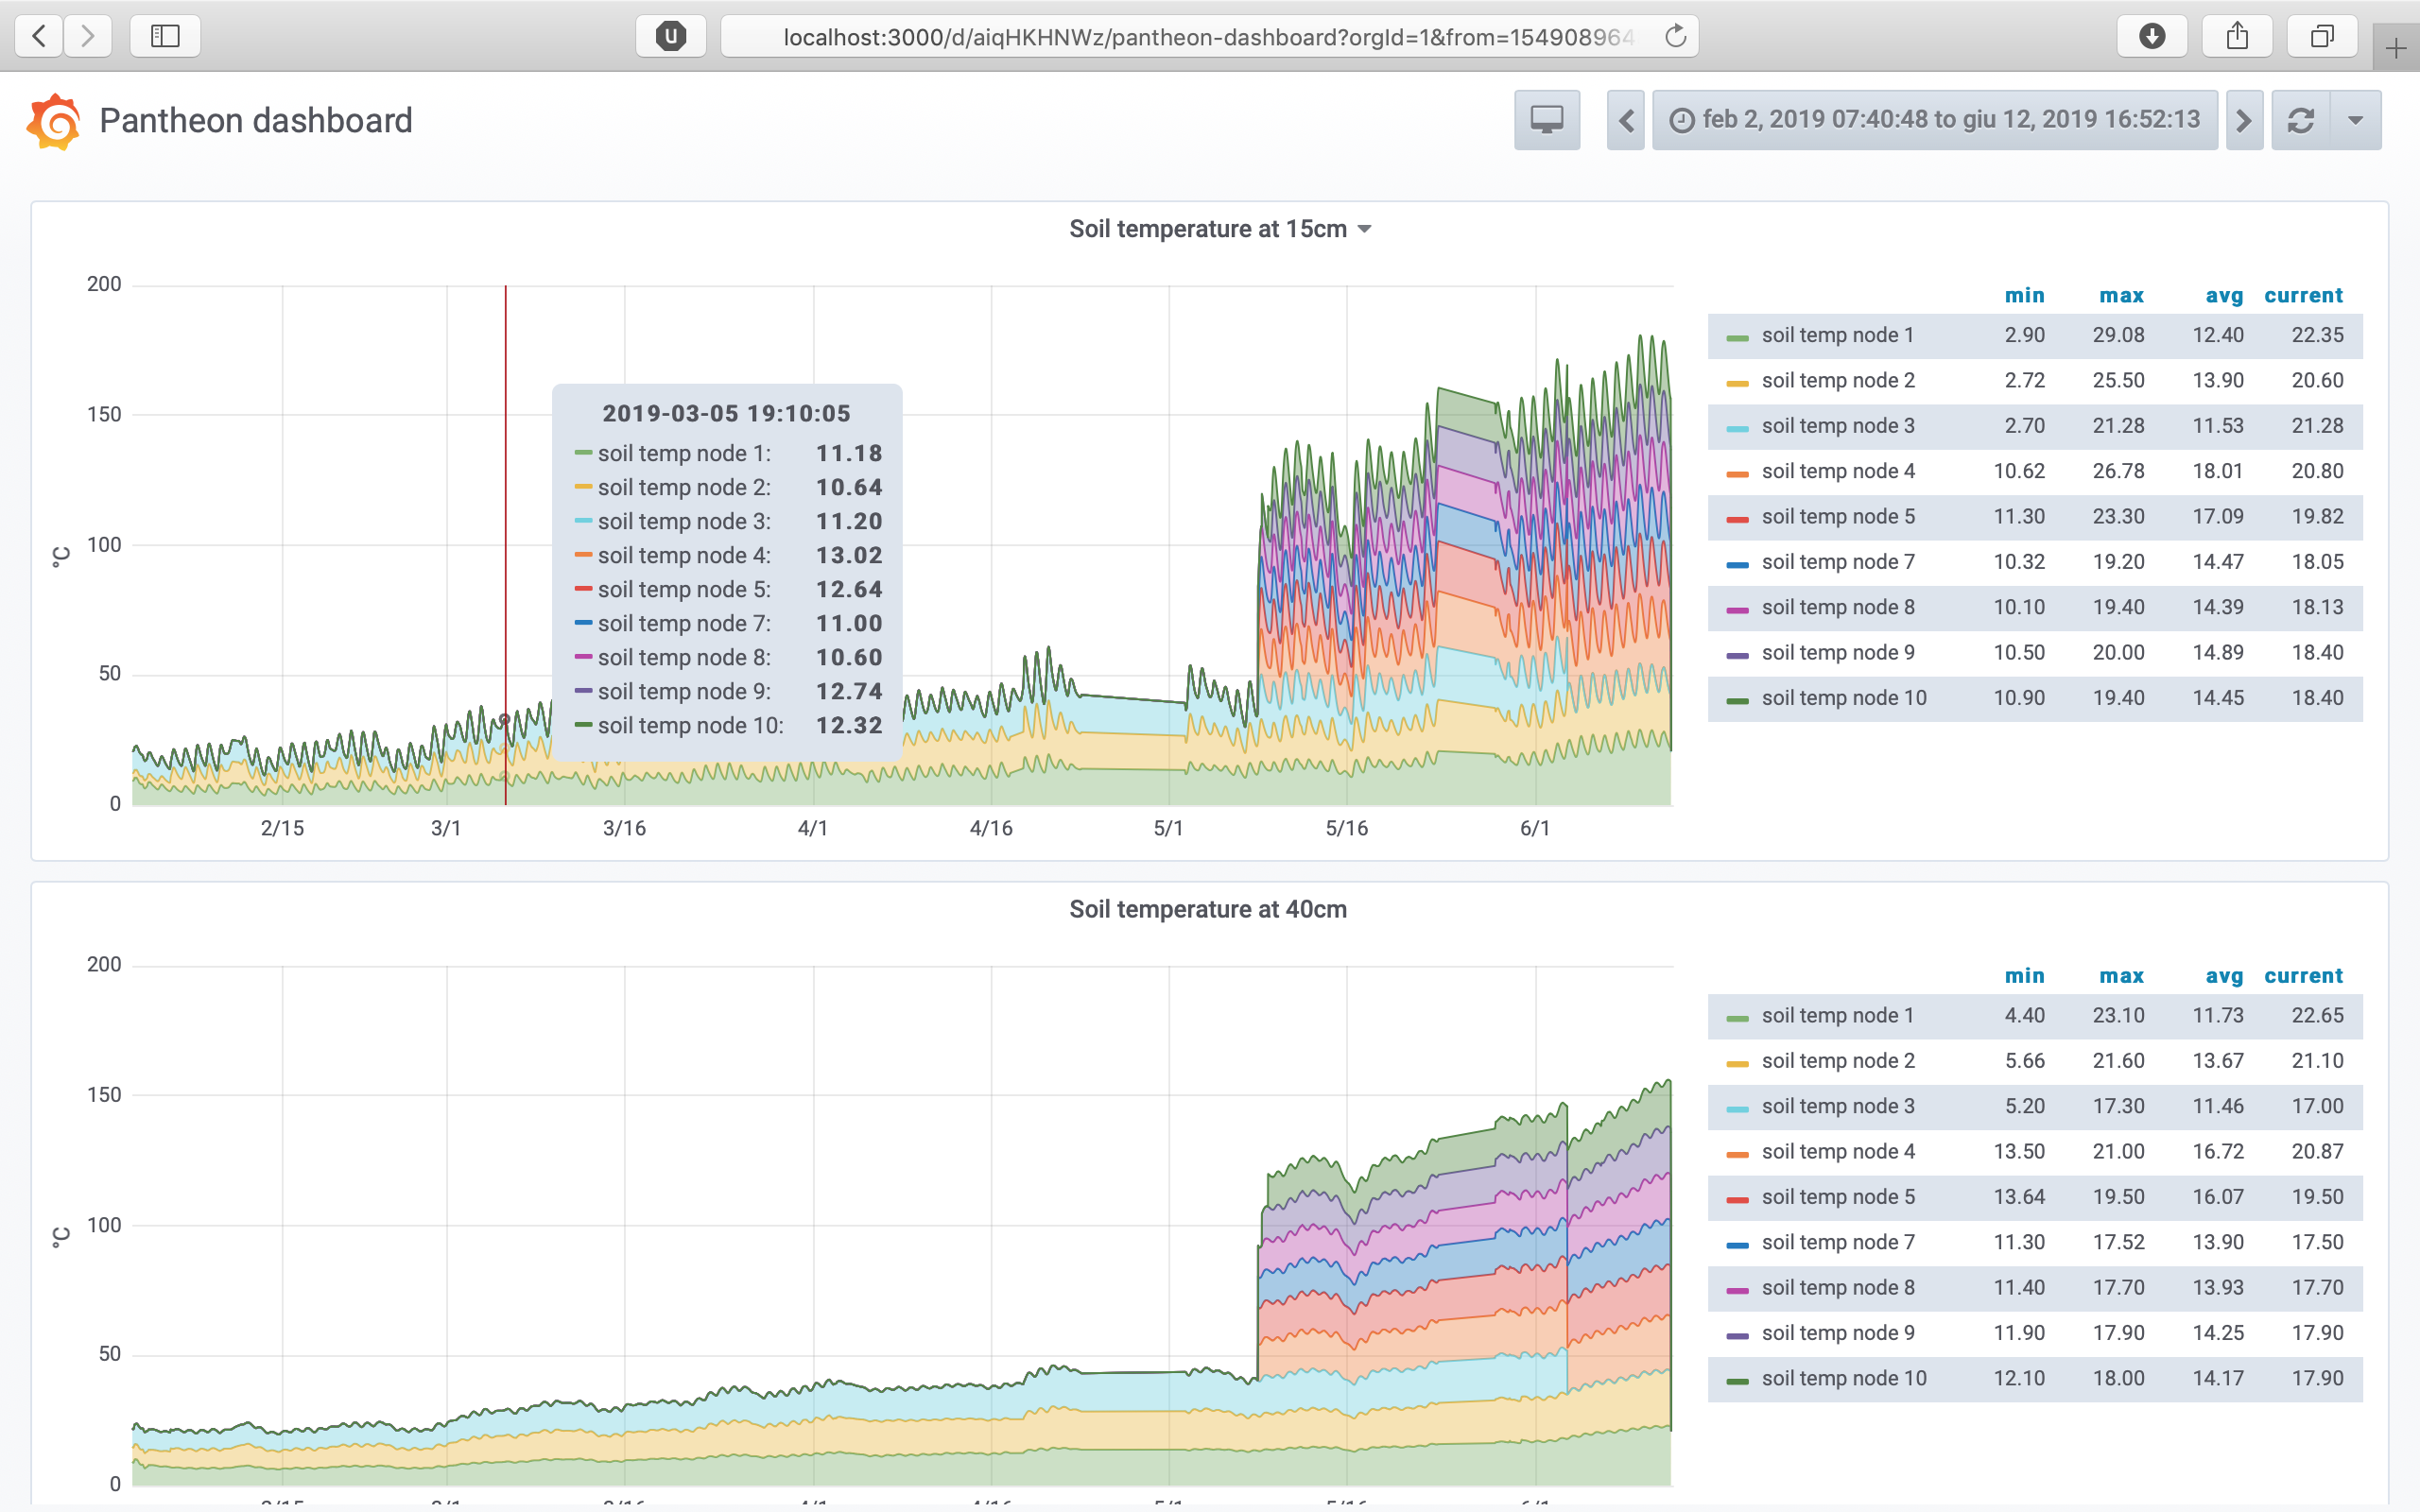
\includegraphics[width=1\textwidth]{grafana-dashboard-1}
\caption{Porzione della dashboard realizzata con Grafana che mostra la temperatura del suolo registrata dai vari sensori}
\label{fig:grafana-dashboard-1}
\end{figure}

\begin{figure}[ht]
\centering
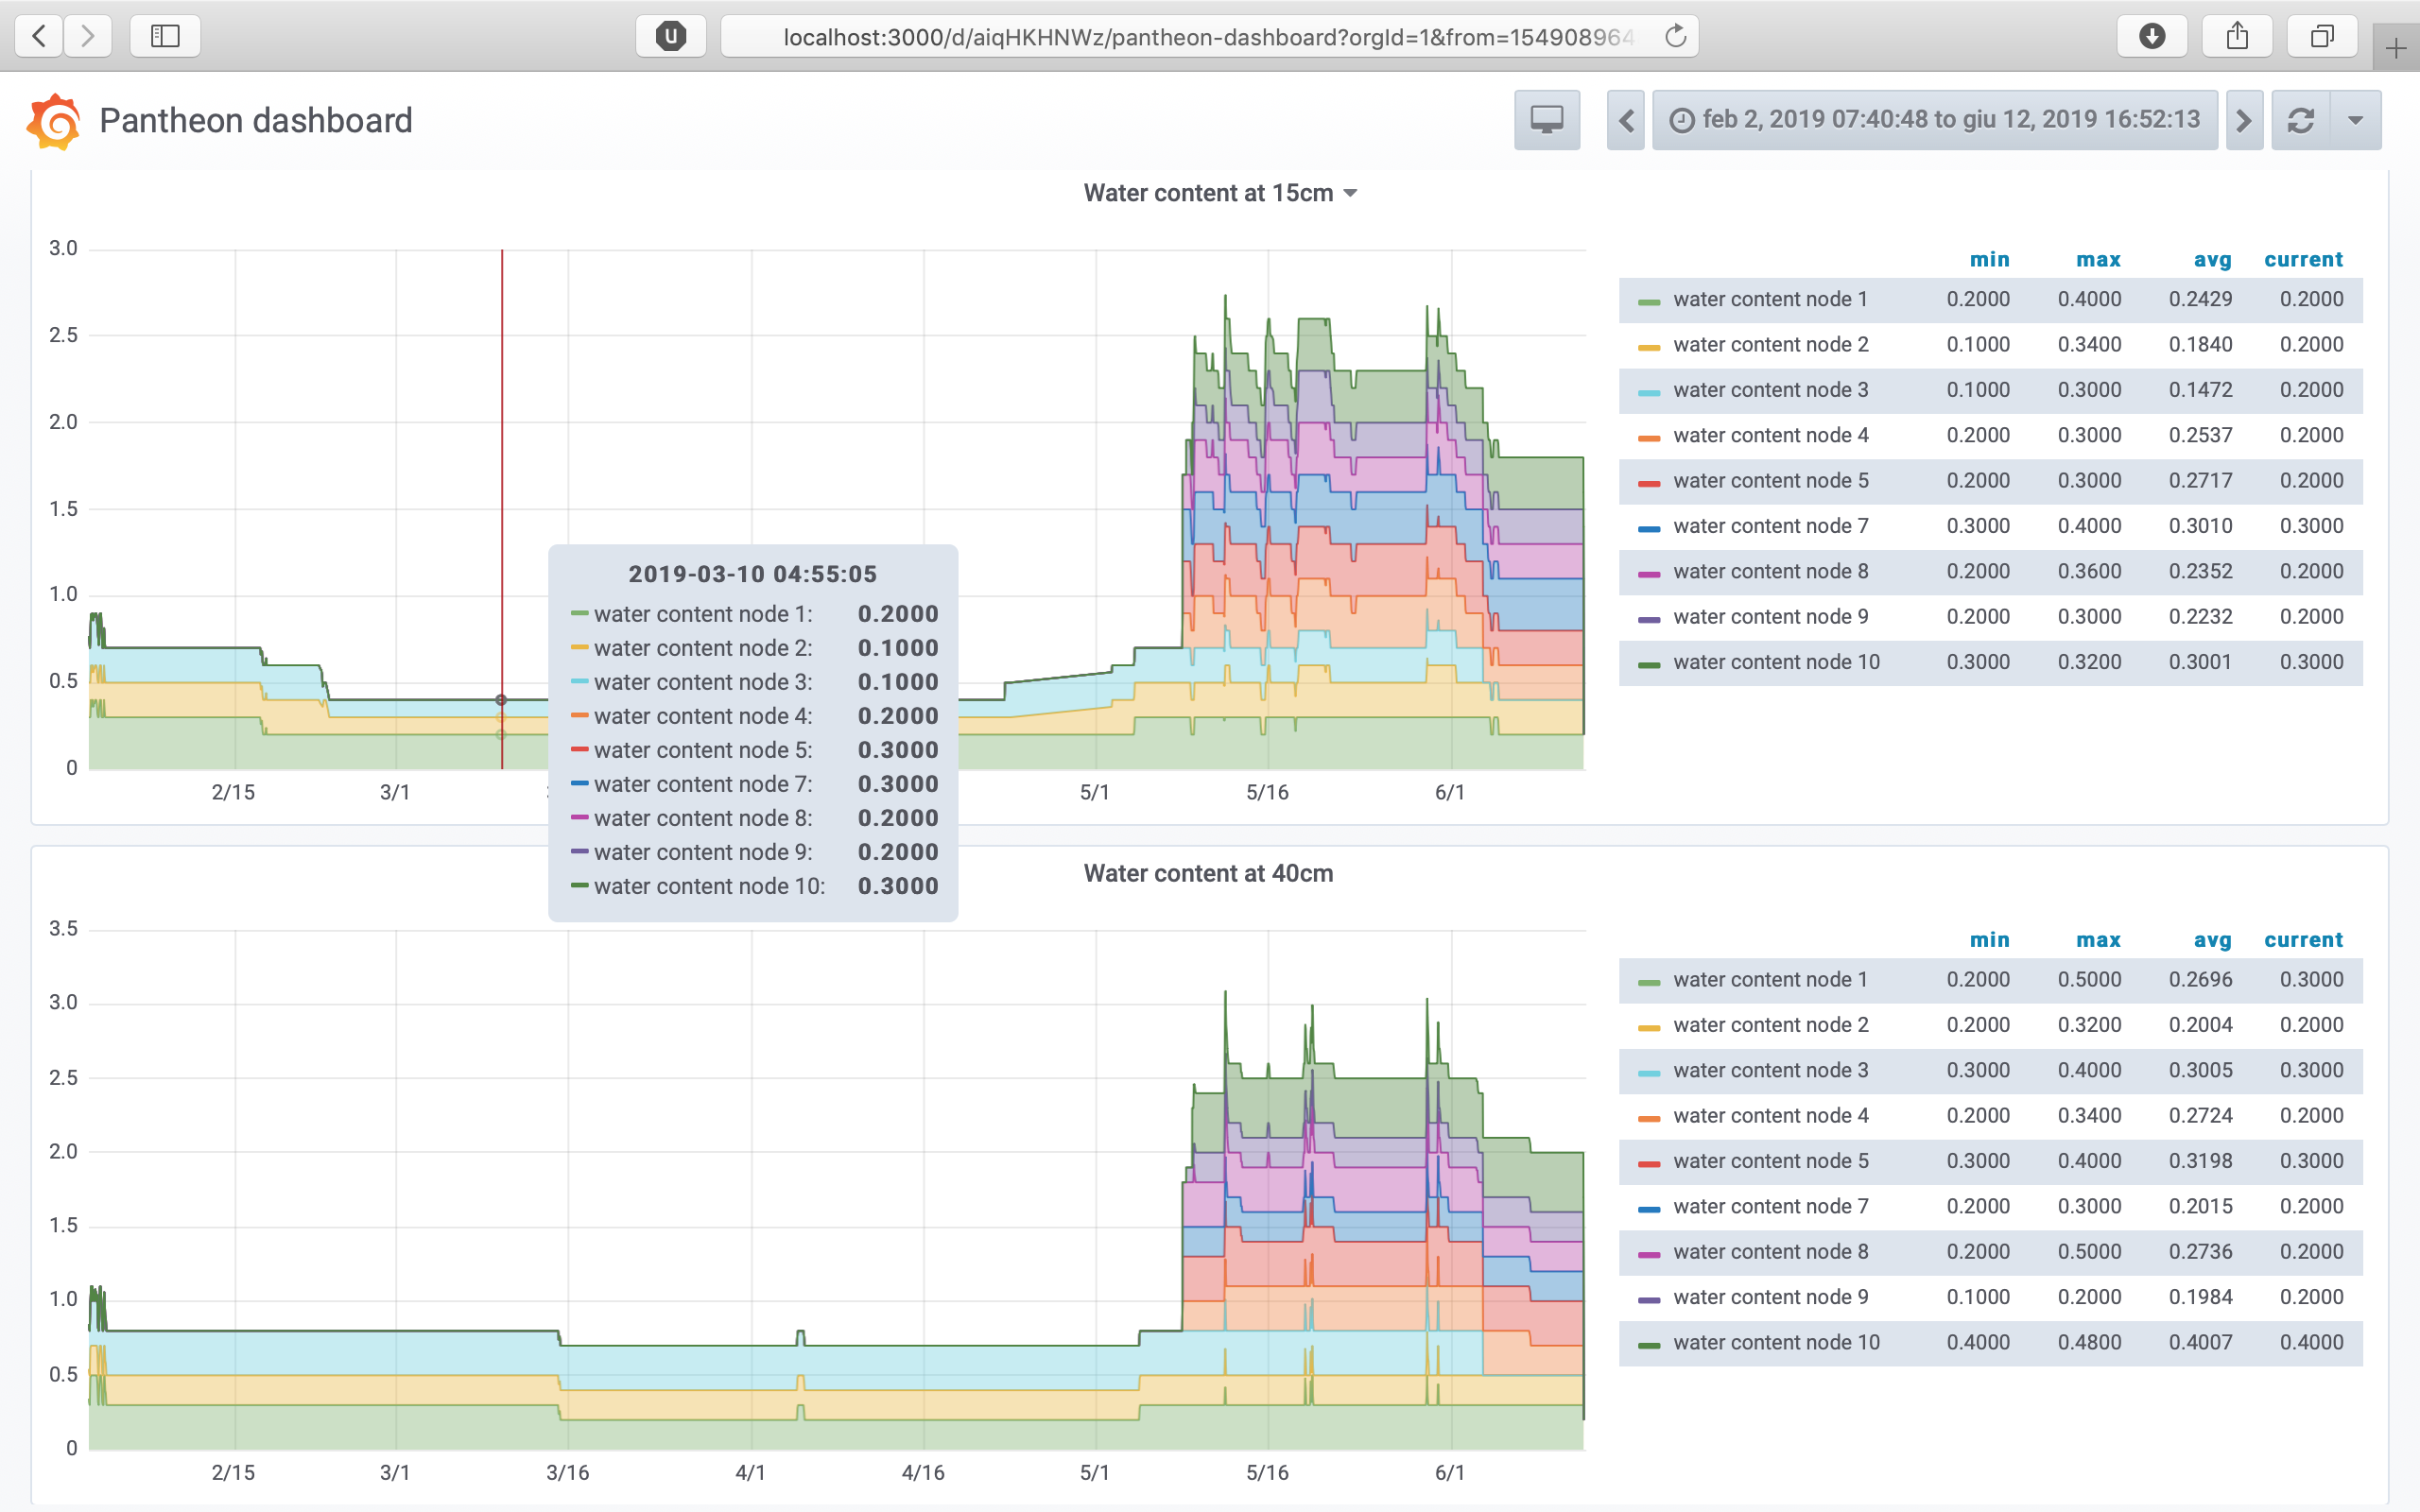
\includegraphics[width=1\textwidth]{grafana-dashboard-2}
\caption{Porzione della dashboard di Grafana che mostra la quantità d'acqua presente nel terreno registrata dai vari sensori}
\label{fig:grafana-dashboard-2}
\end{figure}

Notare come per ogni serie temporale presente nella dashboard vengano riportati i valori massimi, medi e minimi (i quali vengono aggiornati ad intervalli di 5 secondi - la frequenza di aggiornamento è configurabile a partire dall'interfaccia grafica di Grafana).